% !TeX root = ./main.tex

% ------------------------------------------------------------------------------------

\chapter[INTRODUCTION]{INTRODUCTION}

Very general introduction why the topic of the thesis is relevant.

Road Safety Scenario in the World and in Brazil.

Urban planning having a crucial role on the road safety in cities.

\section{OBJECTIVES}

In the context of the urban planning practices and road safety management, the main objective of this research is to investigate the influence of demographic, socioeconomic, land use and constructed environment on the speeding practices as a risk factor on the frequency and severity of road crashes. The scenario of the study is the city of Curitiba, capital of the state of Paraná, Brazil. The correlation (or lack of) will be analyzed with the use of the Geographically Weighted Regression statistical model.

With the use of speeding data collected from drivers that participated in a Naturalistic Driving Study (NDS) performed in Curitiba, this investigation aims to contribute to the knowledge of its relationship with variables from the built environment (BE). These BE variables are categorized by \textcite{Ewing2009} in five groups called '5D': density, diversity, design, destination accessibility and distance to transit. In addition to these variables, this study aims to relate the income as a socioeconomic variable to the speeding as well.

As co-benefits in the investigation, this thesis aims to offer some level of insight regarding the development and update of speed control in cities, considering the operational and structural planning guidelines for the road systems and land use. With these factors in mind, it could be possible to present new ideas to the planning practices in Curitiba, regarding mobility plans, master plans and zoning laws.
    

\section{JUSTIFICATION}

The excess of traffic speed performed by vehicles on urban environments are a main risk factor in the chance and severity of road crashes, considering there is great volume of interaction between motorized and vulnerable users \cite{Elvik2009}. Considering the direct relationship between the mobility, the land use patterns and the built environment \cite{DeVos2013}, it is important to investigate these factors in search of improvements in the management process of the road safety. Speeding, which is on the primary causes for traffic crashes \cite{WHO2013} can be better studied and analyzed by the collection of naturalistic data.

Having in mind that most of the traffic crashes and conflicts happens in cities \cite{WHO2018}, as a consequence of the fast process of urbanization in the last decades, it is crucial to create safer conditions in these localities. In Brazil, the management of the mobility is attributed to the municipalities \cite{Brasil1997}. Therefore, the management of road safety, as a task inherent to traffic management, is also an attribution of the municipalities. It is necessary to observe the issues of road safety in cities when conducting the process of urban planning. Having this in mind, it was established laws in which this integration between the planning process by the municipalities and the sustainable mobility are clearly defined: The Statute of the Cities \cite{Brasil2001} and The Law of the Urban Mobility \cite{Brasil2012}.    

The built environment can affect the traffic safety through three main mediators: the traffic volumes, traffic conflicts and traffic speeds - which can directly affect the crash safety and severity in urban environments \cite{Ewing2009}. Traffic crashes are a final outcome of the problems involving the road safety. Therefore, in order to have a method to analyzed the operational conditions of the traffic safety in cities, it can be beneficial to use a intermediate outcome - or a safety performance indicator (SPI) \cite{Bastos2014} - which can be the amount of speeding that occurs across its territory, in addition to the studies that uses the traffic crashes as dependent variables. 

\section{THESIS STRUCTURE}

General composition of the thesis, giving which chapters the reader should expect

Write this part after completion of chapters 2 and 3

% ------------------------------------------------------------------------------------

\chapter{LITERATURE REVIEW}

%Develop a review based on the theme of the thesis (road safety, city planning, land use ...)

%Identify a gap in the literature I want to fill (Most of the works analyses the road accident as a response variable), assessing the importance of this thesis.

\section{ROAD SAFETY SCENARIO}

% 1. Road safety in the world: OECD countries, the three hypothesis involving development and road safety, how LMIC countries can overcome road safety problems and learn from OECD, relate to socioeconomic development. One of the main death causes in the world (WHO)

Road traffic crashes around the world claims more than 1.3 million lives in each year, representing the eighth leading cause of deaths and causing up to 50 million injuries. Low and middle income countries (LMICs), including Brazil, suffers from traffic crashes death rates three times higher when compared to developed countries \cite{WHO2018}. The increasing number of traffic crashes deaths on LMICs is a consequence of a intense process of motorization that has been occurring in the last decades. To \textcite{Bhalla2016}, it is important to understand the evolution of road safety management on OECD developed countries in order to overcome the road safety problems in LMICs. 

%% present the three hypothesis involving development and road safety and how lmics can overcome this

Over the last century, the road safety performance of the OECD countries showed a consistent pattern. The road traffic death rate (per 100,000 population) in these countries were rising until the 1960s, as seen in \autoref{fig:oecd}. After this period, all countries showed a declining pattern, whilst the LMICs still had a rising pattern due to the rapid growth in their motor vehicle fleets. This behavior of rising and declining trend on the road traffic death rate could be explained by three phenomenons: economic determinism, risk substitution and a political shift in the road safety paradigm \cite{Bhalla2016}.

\begin{figure}[!htbp]
    \centering\footnotesize
    \captionsetup{font=footnotesize}
    \caption{ROAD TRAFFIC RATES IN OECD COUNTRIES}
    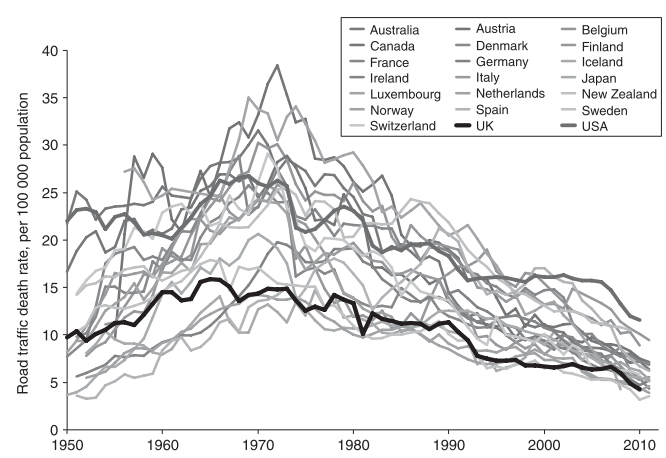
\includegraphics[width=0.8\textwidth]{fig/oecd.png}
    \label{fig:oecd}
    \par SOURCE: \textcite{Bhalla2016}.
\end{figure}

In the scope of economic determinism, the road traffic deaths are defined as a process related to the country development. The rising pattern is associated with the increase in motorization, and the falling happens after a certain level of development, where the countries have the means to start investing in road safety. But this hypothesis has some flaws. This creates an impression that LMICs are not able to invest in road safety before becoming full developed, which is inaccurate. Also, this idea shifts the focus on investment in direct interventions, encouraging the countries to focus on income growth as a strategy for road safety \cite{Bhalla2016}.

As the mobility in general becomes more motorized towards the use of the car, pedestrians starts transitioning into car users. This circumstance is known as risk substitution, where the increase in car users occurs at the same time as the number of pedestrians declines, lowering the exposure to more severe road traffic injuries like the collision between cars and pedestrians and lowering the number of road traffic deaths. But this phenomenon can be imprecise when considering the motorization of LMICs, in which mass transit, motorcycles and other non motorized transports have a greater role on the vehicle fleet \cite{Bhalla2016}.   

A factor that explains this pattern in a more precise way is the political shift in the road safety paradigm that happened on the OECD countries. Before the 1950s, the belief that drivers were the only responsible for the road crashes lead the discussions regarding road safety. Therefore, most of the interventions in road safety management ignored the design and development of the build environment and the vehicles. Between the 1960s and the 1970s, OECD countries started to regulate transport in order to tackle the road safety problems that were rising, establishing new laws and road safety management institution on national e local levels. \cite{Bhalla2016}. Analyzing the road safety data from Brazil, it is possible to correlate the actual stage with what the OECD countries passed during the 1970s.

% 2. Road Safety historic in Brazil. Death rates evolution ...

%% Brazil standing, absolute value for 2019 (WHO)

 According to \textcite{WHO2018}, it was predicted that Brazil would had a road traffic mortality rate (number of deaths per 100,000 inhabitants) of 22.5 in 2016, the highest rate between the south american countries. In 2019 (the last entry available by \textcite{MinistryofHealth2020}), road crashes were responsible for 31.945 deaths. Considering the Decade of Action for Road Safety 2011-2020 \cite{WHO2011}, Brazil will reach the goal of reducing the road traffic deaths in half (comparing to the number projected for 2020, in case of a rising trend in deaths) by the end of the 2010s. \autoref{fig:br_abs} has the time series of road traffic deaths in the last decades.  

%% Plots with absolute values as well.

\begin{figure}[!htbp]
    \centering\footnotesize
    \captionsetup{font=footnotesize}
    \caption{ROAD TRAFFIC DEATHS ON BRAZIL}
    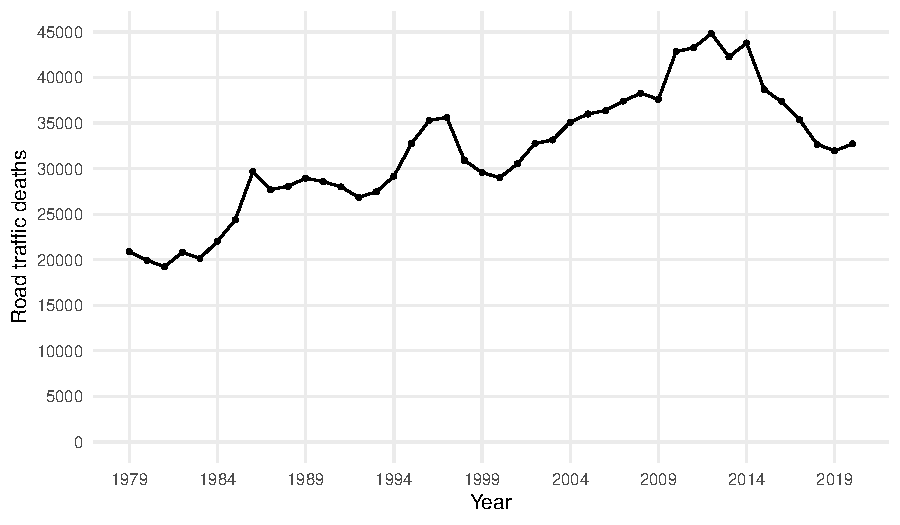
\includegraphics{fig/brazil_abs.pdf}
    \label{fig:br_abs}
    \par SOURCE: The Author, based on \textcite{MinistryofHealth2020}.
\end{figure}

%% Situation regarding the Decade of Action

The year of 1979 is the earliest official data entry available. Starting in the 1980s, there is a overall rising trend in the numbers of road traffic deaths that reach its peak in 2012, then it starts declining. In 2010, the year before the Decade of Action, Brazil had 42,844 deaths and reached the max value in 2012: 44,812 road traffic deaths. Almost at the end of the decade the number of deaths declined, reaching 31,945. The next plot (\autoref{fig:br_mort}) shows the mortality rate in Brazil, considering the same time span. In general, it follows the same pattern of the absolute road traffic deaths.

%% Show mortality, gdp and motorization as well; correlation between gdp and motorization (Bastos, 2014; Ferraz et al, 2012)

\begin{figure}[!htbp]
    \centering\footnotesize
    \captionsetup{font=footnotesize}
    \caption{ROAD TRAFFIC MORTALITY RATE ON BRAZIL}
    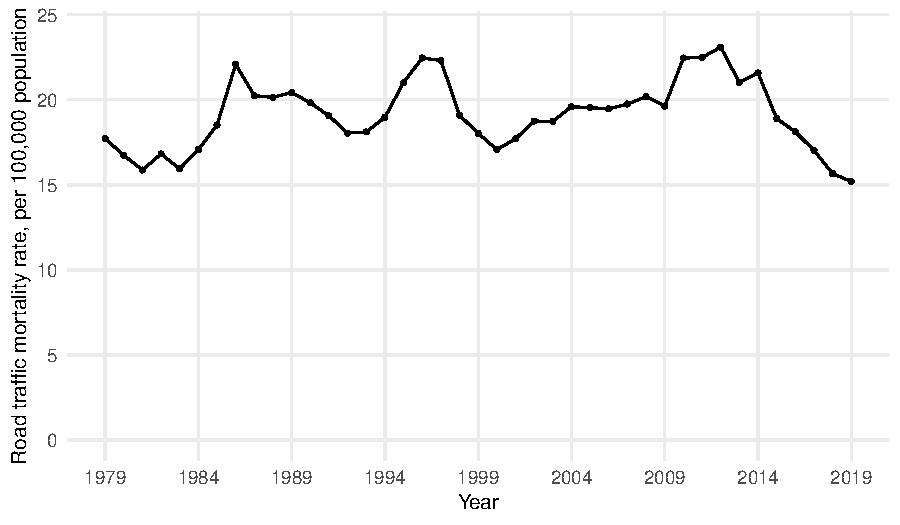
\includegraphics{fig/brazil_mort.pdf}
    \label{fig:br_mort}
    \par SOURCE: The Author (2021), based on \textcite{MinistryofHealth2020} and \textcite{MinistryofHealth2021}.
\end{figure}

%% Compare Brazil to other countries (who, 2016 - just numbers)

The maximum registered mortality rate is 23.1 deaths per 100,000 inhabitants in 2012, the same year which Brazil reached its maximum value for absolute road traffic deaths. Since then the mortality rate has been declining, reaching a rate of 15.2 deaths per 100.000 inhabitants in 2019. In comparison to the OECD countries (\autoref{fig:oecd}), Brazil presented a strong declining pattern a few years later, after the 2010s. Another indicator that considers the exposition to traffic hazards is the fatality rate - number of deaths per 10,000 vehicles (\autoref{fig:br_fatal}). The oldest entry of fleet size in the \textcite{DENATRAN2020} database is 1998.

\begin{figure}[!htbp]
    \centering\footnotesize
    \captionsetup{font=footnotesize}
    \caption{ROAD TRAFFIC FATALITY RATE ON BRAZIL}
    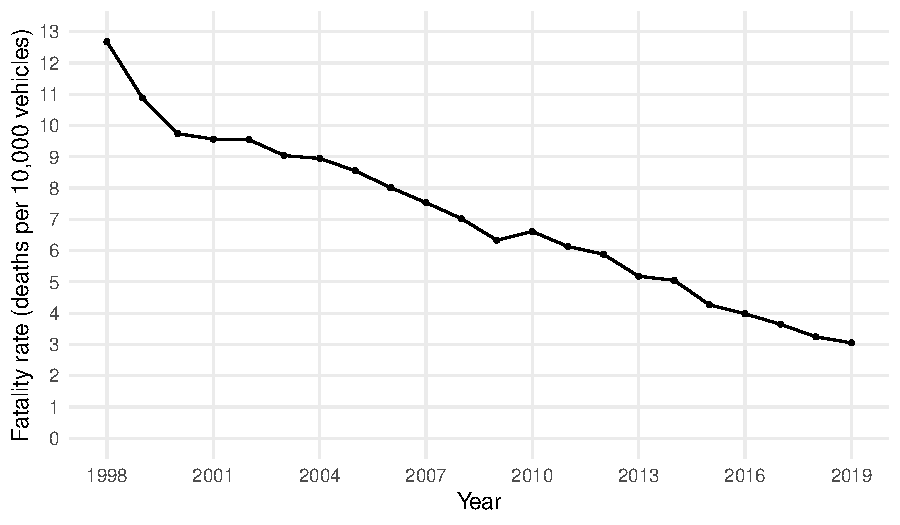
\includegraphics{fig/brazil_fatality.pdf}
    \label{fig:br_fatal}
    \par SOURCE: The Author (2021), based on \textcite{MinistryofHealth2020} and \textcite{DENATRAN2020}.
\end{figure}                                

Between 1998 and 2019 there is a declining pattern in the fatality rate, starting with 12.7 deaths per 10,000 vehicles in 1998 and ending with 3.0 in 2019, representing a reduction of 76\%. This declining pattern can be explained by the continuous rise of the motorization rate (\autoref{fig:br_motor}). In 1998, the motorization rate was 151 vehicles per 1,000 population, increasing to the rate of 499 in 2019. The motorization can be defined as one indicator of the development un the country. Considering the motorization stages defined by \textcite{Jorgensen2005}, Brazil can be classified nowadays with a exploding motorization. 

The first stage of motorization - developing motorization - occurs when a country have a motorization rate between 50 and 100 vehicles per 1,000 inhabitants. This first stage happened in Brazil before 1998. The explosion of the motorization is the second stage, and it happens with a motorization rate of between 300 and 400. The third and last stage is the saturation, and occurs when the motorization rates reaches more than 400 and its tendency stops rising \cite{Jorgensen2005}. Although Brazil has a present motorization rate above 400, it is plausible to affirm that the country still hasn't reached the stage of saturation, considering that the rates are still in a rising pattern. 

%% Insert motorization plot

\begin{figure}[!htbp]
    \centering\footnotesize
    \captionsetup{font=footnotesize}
    \caption{MOTORIZATION RATE ON BRAZIL}
    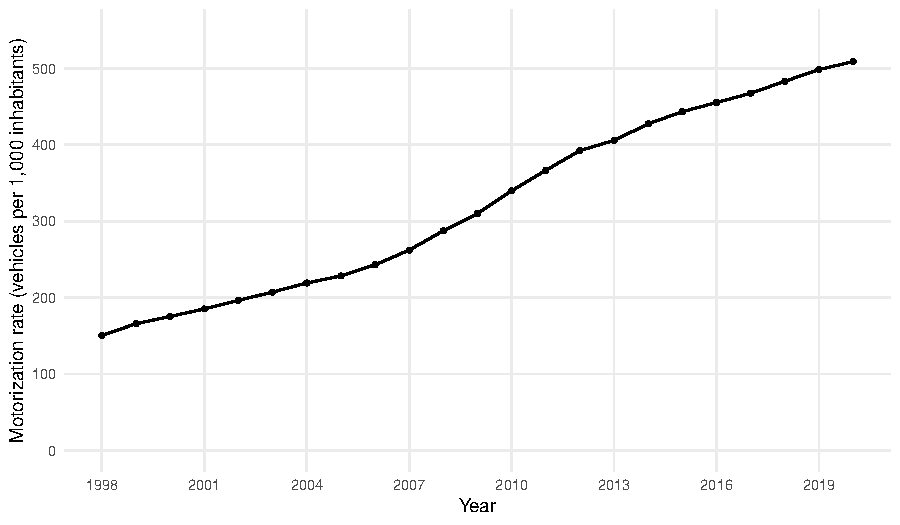
\includegraphics{fig/brazil_motor.pdf}
    \label{fig:br_motor}
    \par SOURCE: The Author (2021), based on \textcite{MinistryofHealth2021} and \textcite{DENATRAN2020}.
\end{figure} 

%% Explain the relation between deaths and economic situation in Brazil (Ferraz, search in Tiago doctor thesis, livro onsv)

%% Historic of interventions: CTB, 1998; Lei seca, 2012

In the 1970s, Brazil have undergone through a intense development in the car industry, lowering the price of the vehicles and increasing the development of road infrastructure in cities and rural areas, impacting directly in the rise of the motorization in the country \cite{Vasconcellos2013}. To \textcite{Harvey1982}, this incentive to motorization created a urban environment that looked to answer the increasing demand of car use. This process lead to worse safety conditions in brazilian cities, specially non motorized users in the road system.   

The variation in the number of road traffic deaths and road traffic mortality heavily influenced by the socioeconomic development and political landscape \cite{Ferraz2012}. The country had different economical situations between the 2000s and the 2010s. In the period of 2000-2010, Brazil had a continuous growth in the economy, which reflected on the rising pattern of the road traffic deaths and road traffic mortality rates. After the 2010, the country entered in a economic recession, leading to the reduction of these numbers \cite{Bastos2020}. Focusing on the area of study, the road traffic deaths in Curitiba are presented in \autoref{fig:cwb_abs}.   

%% Now focusing on the area of study, the city of Curitiba ...

%% death rates in curitiba (compare to others capitals) -- fatality rate, mortality rate, motorization, gdp)

\begin{figure}[!htbp]
    \centering\footnotesize
    \captionsetup{font=footnotesize}
    \caption{ROAD TRAFFIC DEATHS ON CURITIBA}
    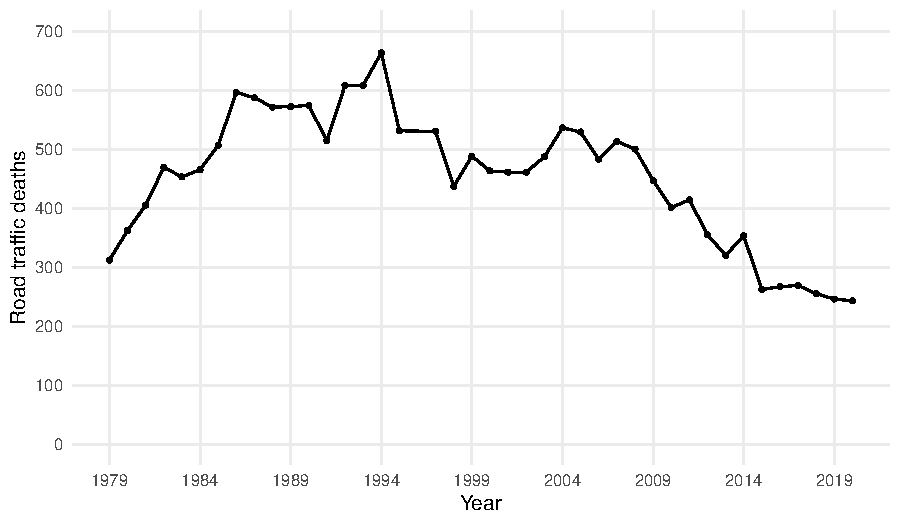
\includegraphics{fig/cwb_abs.pdf}
    \label{fig:cwb_abs}
    \par SOURCE: The Author (2021), based on \textcite{MinistryofHealth2020}.
\end{figure}  

The tendency of road traffic deaths presented a rising pattern between 1979 and 1994, starting with 312 deaths and reaching a maximum of 663 deaths. Overall, the pattern of the time series started declining after 1995, ending with a minimum value of 246 in 2019. Following the brazilian trend, Curitiba's motorization rate kept rising in the last decades. The increase in motorized transit can lead to more exposition to traffic crashes and injuries, in case road safety interventions are not implanted correctly. The plot in \autoref{fig:cap_motor} compares the motorization rate between all brazilian states capital cities.    

\begin{figure}[!htbp]
    \centering\footnotesize
    \captionsetup{font=footnotesize}
    \caption{MOTORIZATION RATES ON BRAZILIAN STATES CAPITAL CITIES, IN 2019}
    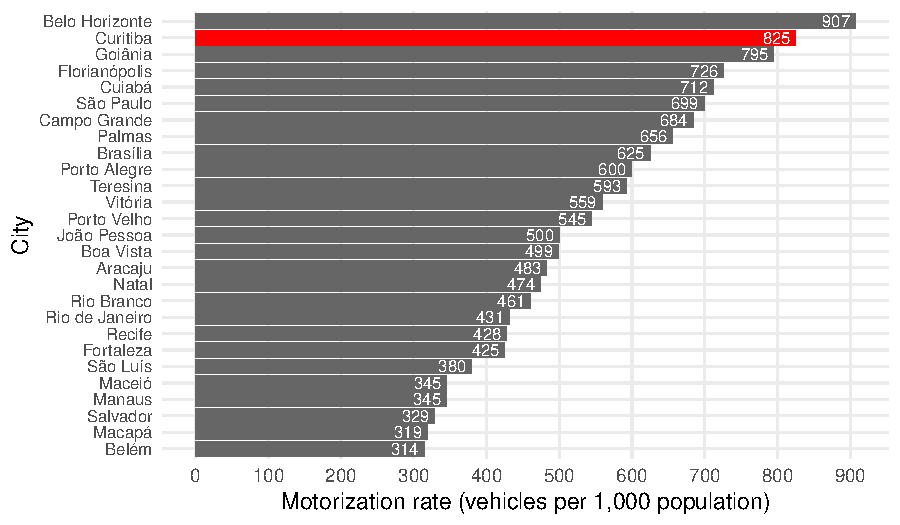
\includegraphics{fig/cap_motor.pdf}
    \label{fig:cap_motor}
    \par SOURCE: The Author (2021), based on \textcite{MinistryofHealth2021} and \textcite{DENATRAN2020}.
\end{figure}   

Curitiba was, in 2019, the second most motorized capital in Brazil, with a motorization rate of 825 vehicles per 1,000 population, higher than the brazilian average, losing only to Belo Horizonte, which presented a motorization rate of 907 vehicles per 1,000 population. When comparing the road traffic mortality rate (\autoref{fig:cap_mort}), Curitiba stays in the 13th place with 12.7 deaths per 100,000 inhabitants, below the brazilian average of 15.2 in 2019. The lowest value of road traffic mortality rate belongs to Rio de Janeiro, presenting a rate of 5.7 deaths per 100,000 population, and the highest belongs to Palmas, with a alarming rate of 36.4. 

\begin{figure}[!htbp]
    \centering\footnotesize
    \captionsetup{font=footnotesize}
    \caption{MORTALITY RATES ON BRAZILIAN STATES CAPITAL CITIES, IN 2019}
    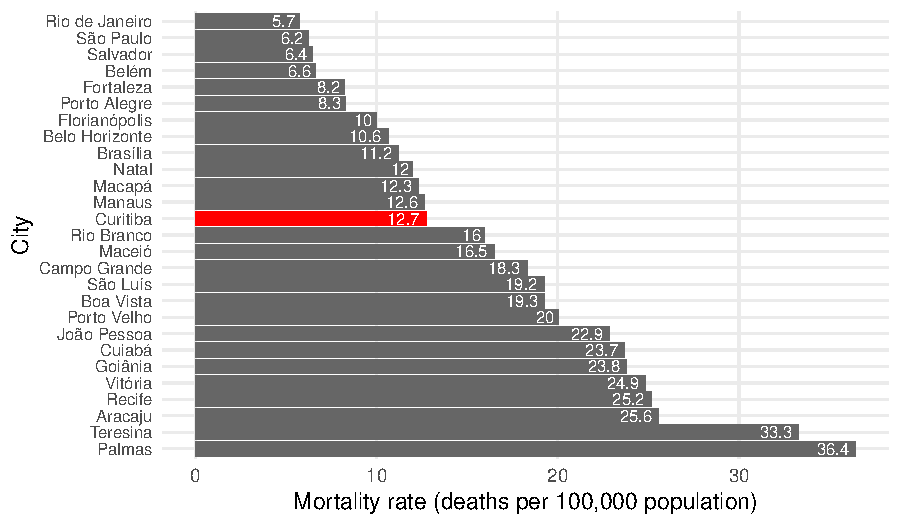
\includegraphics{fig/cap_mort.pdf}
    \label{fig:cap_mort}
    \par SOURCE: The Author (2021), based on \textcite{MinistryofHealth2020} and \textcite{MinistryofHealth2021}.
\end{figure}  

Considering the fatality rate as a road safety performance indicator, \autoref{fig:cap_fatal} plot shows that Curitiba have the 6th best performance, with a fatality rate of 1.5 deaths per 10,000 vehicles. São Paulo is the capital with the lowest fatality rate (0.9) and Recife has the highest one (5.9). Observing the fatality rate in Brazil in the same period (3.0), Curitiba is below the country average, with exactly 50\% less deaths per 10,000 vehicles. Road traffic crashes and its related injuries have become a serious health problem across brazilian cities. As motorization increases, the number of conflicts and possible crashes increases as well.

\begin{figure}[!htbp]
    \centering\footnotesize
    \captionsetup{font=footnotesize}
    \caption{FATALITY RATES ON BRAZILIAN STATES CAPITAL CITIES, IN 2019}
    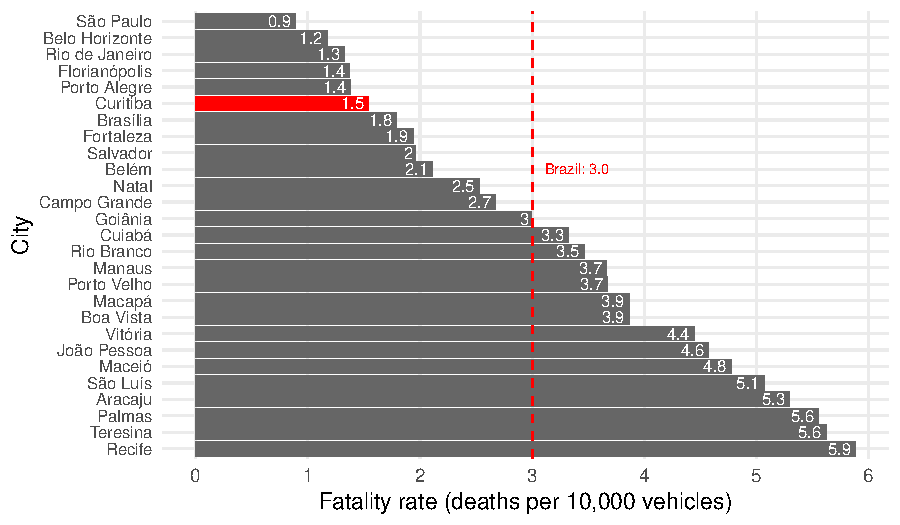
\includegraphics{fig/cap_fatal.pdf}
    \label{fig:cap_fatal}
    \par SOURCE: The Author (2021), based on \textcite{MinistryofHealth2020} and \textcite{DENATRAN2020}.
\end{figure} 

%% Compare curitiba to other international cities (ENBARQ) and another countries (WHO, 2016, just numbers)

%When comparing Curitiba's mortality rate in 2019 (12.7) to other countries, 

% 3. Road safety as a public health problem, as a result of the interaction between human, environmental and vehicle factors

%% How to tackle this problem. 

%% Two scales of dimensions: parts involved and crashes timeline. 

%% Hadden matrix, relating to the present thesis. 

Capable interventions in road safety needs to consider traffic deaths and injuries as serious public health problems. Therefore, its control must follow the principle as control of any other public health problem. Road traffic injuries are the result of a complex interaction of multiple factors. These factors can involve human, environmental and vehicle factors, in addition to sociological, psychological, physical and technological factors present the process of traffic crashes. As another health problems, it is possible to analyze road traffic injuries considering three different phases in time: pre-crash, during the crash and post-crash \cite{Mohan2016}.

These distinct phases of time and factors of road traffic crashes can be arranged into a matrix created by \textcite{Haddon1980} in order to map all events related to a injury. Named after its inventor, the Haddon matrix (\autoref{fig:haddon}) consists of two dimensions: one for the time aspect of the event and a second one representing three main discrete factors: human, vehicle and environment. Crossing each step of both dimensions sets nine cells, in which can be made a list of countermeasures to control the damage or to prevent a possible incident, associating these measures to each pair of factors. 

\begin{figure}[!htbp]
    \centering\footnotesize
    \captionsetup{font=footnotesize}
    \caption{HADDON MATRIX}
    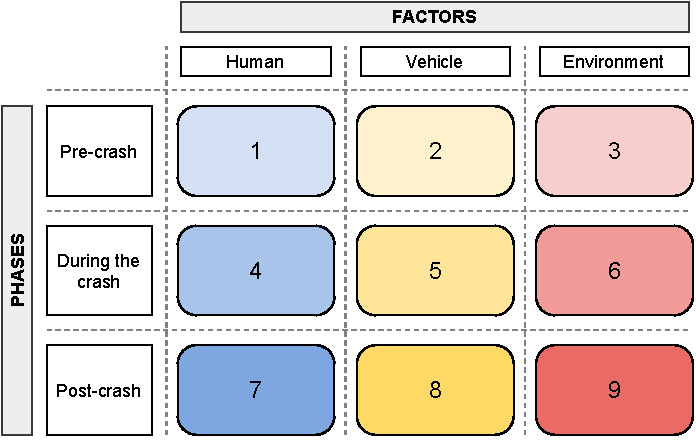
\includegraphics{fig/haddon.pdf}
    \label{fig:haddon}
    \par SOURCE: The Author (2021), based on \textcite{Haddon1980}.
\end{figure} 

Cells 1, 2 and 3 contains measures towards the prevention of crashes. On a road traffic crash scenario, cell 1 considers the behavior (aggressive driving, driving under influence, distraction) and training of the road users (pedestrians, drivers, motorcyclists and cyclists), cell 2 presents safety interventions related to the vehicles (use of daylight headlights, speed control systems, etc.) and cell 3 contains all elements of the road infrastructure the and build environment that influences directly into the occurrence of this event. Cells 4, 5 and 6 comprehends measures that can reduce the severity during the occurrence of a crash event.

In cell 4 there are measures that include the use of seat belts, helmets and protective clothing. Cell 5 can consider the crashworthiness and safety design of the vehicles and cell 6 includes elements (or lack of elements) that can influence the severity in case of a collision (guard rails, concrete barriers, street furniture, etc.). In the last row are included the measures related to the control and treatment of injuries after the event. Cell 7 presents the treatments related to the victims (hospital care and rehabilitation), cell 8 contain measures related to the safety systems of a vehicle and cell 9 can consider the general management of a crash scene \cite{Mohan2016}. 

% 4. How these problems are divided between roadways and urban environments.

The road safety problems that happens on urban environments may differ from the ones that happens in major roadways. Even with lower operating speeds, the quantity of conflicts in urban road systems can be considerable higher when comparing to rural roadways, considering the quantity of different motorized and non-motorized transport modes that uses the infrastructure in the same time. Consequently, it is essential to follow requirements for a safe infrastructure. Three main ones are functionality, homogeneity and recognition \cite{SWOV2003}. Each road on a network needs to have a specific function (balance between mobility and access), with traffic distribution working as intended. Homogeneity consists in reducing the points of conflict between transport modes with great difference of mass and speed. Finally, the situations on traffic should have a level of predictability, passing what behavior should be expected from the road users.

% 5. Main risk factors (WHO, WRI): MPU, seat belt, DUI, speeding (inappropriate speeds (ferraz): focus on urban environments (connect to Haddon), elvik

In order to reduce road traffic crashes and possible consequent injuries or deaths, it is relevant to consider the main risk factors that causes and intensify these events. According to \textcite{WHO2004}, risk in road traffic can be classified into four elements which are directly influenced: exposure, crash involvement, crash severity and post-crash severity. The risk factors that can be classified in these elements also can be distributed within the Haddon matrix as well \autoref{fig:haddon}. The main risk factors related to the protection of the user consists in the usage of seat belts, helmets, air bags, child restraints and helmets. Focusing on the behavioral factors, the main ones are driving under influence of alcohol and another drugs (DUI), distraction and inattention \cite{Shinar2017}.

% 6. Create a hook to the speeding section (next one)

The excess of speed and the speed differential in urban environments are two risk factors that affects the chance of traffic crashes occurrence and the severity of theses crashes. Speeding is a complex phenomenon with multiple causes, consequences and methods of prevention. Given its complexity and spotlight in this thesis, this risk factor will be discussed in the next section (\ref{speeding}). 

\section{SPEEDING} \label{speeding}

% 1. Intro (WHO)

%% WHO, 2013 (speeding is the main cause ...)

Speeding is one of the primary global causes of road traffic fatalities, affecting two main dimensions: probability and severity \cite{WHO2013}. The increase in speeds of vehicles is directly correlated to the increase in the occurrence of crashes and its average severity, hence, strongly related to the road safety \cite{Mohan2016a}. Another speed-related risk factor is the speed differential, which is the speed deviation from the average operating speed \cite{Shinar2017}. \textcite{Ferraz2012} defines speeding as a inappropriate speed, leading to more conflict and crashes in certain traffic conditions. 

% 2. Speeding consequences

%% Haddon matrix and speeding

%% Mohan (cap 9) - reaction time, breaking distance and impact energy

%% Ashton

The excess of speed can influence three main factors in the occurrence of a traffic conflict: reaction time, braking distance and force of impact, which is directly correlated to the severity of injuries \cite{Mohan2016a}. Reducing the speed helps the driver to increase its reaction time, also helping the driver to take a correctional action to anticipate crashes \cite{Elvik2009}. Regarding the braking distance, lower speeds reduces the distance necessary to fully stop the vehicle. \autoref{fig:braking} shows the reaction time of a vehicle added to the braking distance, resulting in the distance travelled by the vehicle. The dashed line represents a pedestrian standing 35 meters from the traveling vehicle. 

\begin{figure}[!htbp]
    \centering\footnotesize
    \captionsetup{font=footnotesize}
    \caption{RELATIONSHIP BETWEEN SPEED AND BRAKING DISTANCE}
    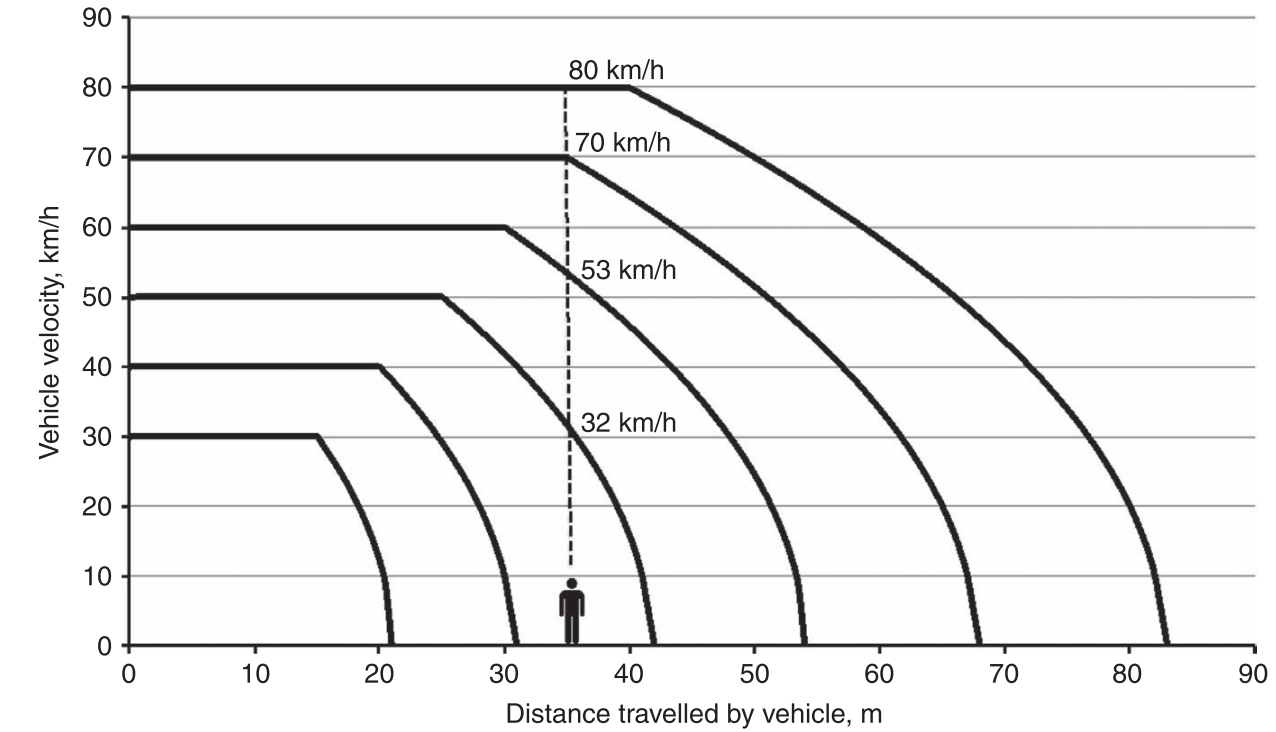
\includegraphics[width=0.8\textwidth]{fig/braking2.png}
    \label{fig:braking}
    \par SOURCE: \textcite{Mohan2016a}.
\end{figure} 

The horizontal lines from the plot shows the cruising speeds of the vehicle before they start breaking, longer lines at higher speeds represents greater reaction times. In this scenario, only speeds equal or below 40 km/h are able to avoid a collision with the pedestrian. As the vehicle speed rises, the impact speed rises as well. This leads to the increase in force of impact between vehicles and pedestrians. The severity of injuries sustained by pedestrians depends on the energy of impact - the kinetic energy transferred to the human body. This energy of an object (the vehicle), directly related to its velocity and mass, detailed in the following equation: \begin{align}
    E = 0.5 \times MV^2 \mbox{;}
    \label{eq:energy}
\end{align} where $E$ is the kinetic energy, $M$ is the object's mass and $V$ is the velocity of the object. The plot in \autoref{fig:kinetic} shows the increase in kinetic energy, considering an average car mass of 1,500 kg \cite{Zervas2008} and speeds varying between 0 and 100 km/h. The quantity of energy doubles when the speed changes from 40 km/h to 60 km/h, and almost triples at 70 km/h. This variation shows how the reduction of speed limits can greatly change the energy of impact.

\begin{figure}[!htbp]
    \centering\footnotesize
    \captionsetup{font=footnotesize}
    \caption{RELATIONSHIP BETWEEN SPEED AND KINETIC ENERGY}
    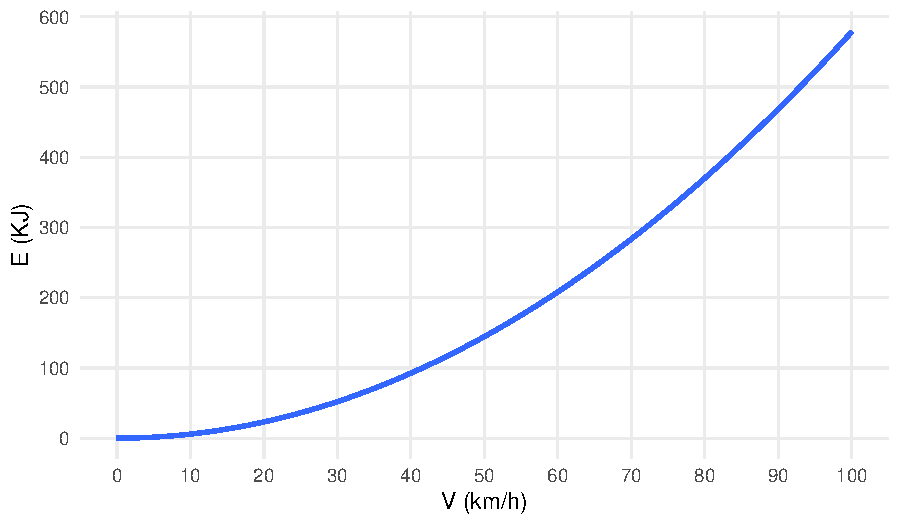
\includegraphics{fig/kinetic.pdf}
    \label{fig:kinetic}
    \par SOURCE: The Author (2021).
\end{figure}

Considering the event of an impact between a front of a car and a pedestrian, \textcite{Ashton1980} presented the relationship between the impact speed and the percentage of fatally injured pedestrians per speed window, represented in the plot of \autoref{fig:ash}. The curve shows how a reduction from 60 km/h to 40 km/h on the speed of impact can reduce the chance of a fatal injury from 90\% to 30\%, approximately. Reducing the speed of impact to 30 km/ will reduce the chance of a fatal injury to approximately 10\%. In general, as the speed of impact rises, the chance of a fatal injury rises too, with a greater variation between speeds of 30 km/h and 60 km/h. 

\begin{figure}[!htbp]
    \centering\footnotesize
    \captionsetup{font=footnotesize}
    \caption{PROBABILITY OF PEDESTRIAN FATALITY AT DIFFERENT IMPACT FATALITIES}
    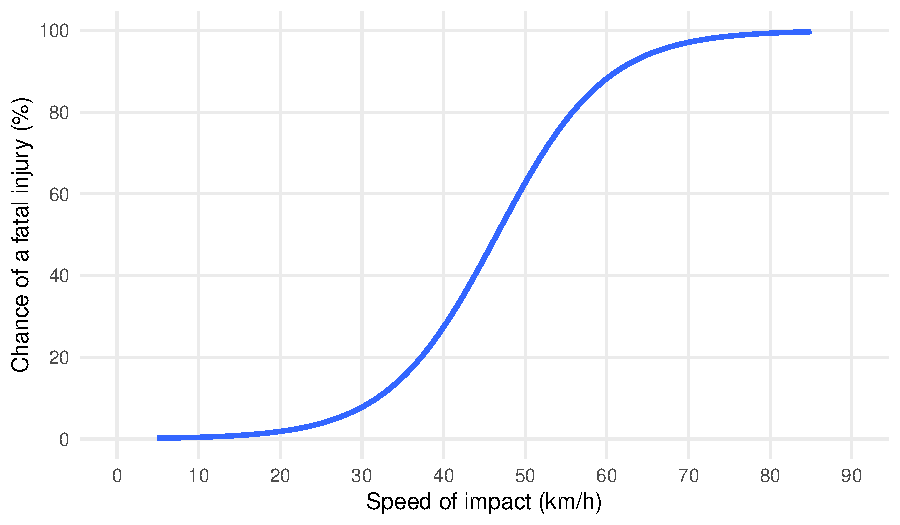
\includegraphics{fig/ash.pdf}
    \label{fig:ash}
    \par SOURCE: The Author (2021), based on data from \textcite{Ashton1980}.
\end{figure}

% 3. Speed management in urban environments: roadways have higher operational speeds, but cities show a bigger interaction between vulnerable and non-vulnerable users, in which lower speeds can represent a risk situation for pedestrians and cyclists.

Theses factors shows the importance of proper speed management in road traffic, specially in urban environments. Roadways have higher operational speeds, but cities contains a more expressive interaction between motorized and vulnerable users, in which lower speeds can still represent a risk to pedestrians and cyclists. One method to manage the operating speed is the enforcement of speed limits. It is recommended a speed limit of 50 km/h in urban arterial roads, and a limit of 30 km/h in roads with a high flow of pedestrians and cyclists \cite{WHO2008}. Reducing the mean speeds can greatly favor the decline in fatal, non fatal and property damage only (PDO) road crashes \cite{Elvik2013}. 

%% ETSC, 1995 (OPAS, 2012 - EMBARQ): recommendations for speed limits. How to enforce? 

The operating and mean speed of the road traffic depends on how the drivers chooses the speed. This choice is related to the power and stability of the user's vehicle, to road and traffic conditions,to  driver's perception of safety, to the level of enforcement, travel motivations, personal characteristics and behavior of other drivers \cite{Mohan2016a, Shinar2017}. Considering all theses factors, it is not effective to rely only on traffic limits to prevent speeding. If the design speed of a road is higher than the speed limit and the road traffic has a low density, it is more difficult to enforce a the desired limit. The difficulty to enforce the speed limits may be higher to LMICs, which have less resources to adopt the proper road designs policies and enforcement levels required to this task \cite{Mohan2016a}. 

% 4. What influences the speed in urban environments? Relate to speed management policies in general (SPEEDING AND ENVIRONMENT).

%% Balance between speed, flow and density. (See Bastos classes and my TCC)

The speed and speed variance are to a certain extent determined by the traffic flow regime \cite{Shinar2017}.  

"In urban areas speeds are controlled by the presence of intersections and the high density of traffic on the roads."

%% WRI

%% Traffic calming measures - WRI

%% Speed differentials

%% countermeasures (shinar, 2007)

% 5. Speeding and behavior. (shinar 2007, elvik et al 2009)

%% How drivers percepts speeding?

%% Drivers choice of speed

%% Richards

% 6. How to collect speeding data: speeding tickets, speed traps (fixed or mobile), researches that considers the accidents reports, behavioral studies, case studies with a local perspective (SPEEDING DATA COLLECTION).

%% Quick pass through speed collection.

%% Hook to NDS

\section{ROAD SAFETY PERFORMANCE AND THE BUILT ENVIRONMENT}

% 1. Introduce the section with Tiwari (2016) and Ewing (2009)

%% Ewing diagram

%% Tiwari 

%% research project item 3.2

% 2. Describe the BE elements. (5D)

%% Tiwari



Present all the available and used indicators. Guide the literature review based on the indicators (which articles are using the same indicators and why - ewing ...)

add ewing, dumbaugh scheme of BE, mediators and safety.

Add description from urban elements (reports passed form Tiago)

Master plan, mobility planning and zoning laws (try to focus on the mobility and road safety, maybe a brief history). --> relating to the previously described elements

\section{NATURALISTIC DRIVING STUDY}

\begin{itemize}
    \item Introduce the Naturalistic Driving Studies as an alternative for the analysis of behavior. Describe multiple international NDS programs, reference the NDS that analyses the speeding. (this part needs to be well described.)
    \item categorize the nds programs and compared with the method used in this work. (maybe construct a table)
    \item Focus on authors that used NDS to study speeding. 
\end{itemize}

\section{GEOGRAPHICALLY WEIGHTED REGRESSION}

Regression analysis is a tool to investigate the dependency between variables and to predict future parameters based on previous ones. This type of statistical analysis can show the relationship between dependent variables (road accidents or speeding) and independent variables (land use, road design etc.) \cite{Lindley1987}. In investigation of the effects of the constructed environment on the occurrence of crashes in urban areas, negative binomial regression is a traditional model used \cite{Wei2013, Zhang2014}. But the quality of this model is limited by the incapacity of analyzing the spatial dependency and heterogeneity expected to happen on road safety factors related to the urban environment \cite{Obelheiro2019}.

% Explain better why GWR is batter and how the previous studies are less precise. 

To overcome this limitation, the Geographically Weighted Regression (GWR) allows the exploration of relationship between variables on a spatial nonstationarity context. The spatial nonstationarity is a scenario where it is assumed that parameters are not constant across the space. In this thesis context, these parameters are the occurrence of speeding across Curitiba's territory. A global regression model may be incapable of explaining the relationship between sets of variables with a acceptable level of precision in this scenario. The GWR model considers that the nature of the model must alter over space to reflect the structure within the data, allowing the actual parameters for each location in space to be modeled and mapped \cite{Brunsdon2010}.

The basic form of GW linear regression is based on the following equation:\begin{align}
    y_i = \beta_{i0} + \sum_{k=1}^{m} \beta_{ik} x_{ik} + \epsilon_i \mbox{;}
    \label{eq:gwr}
\end{align} where $y_i$ is the dependent variable (speeding) at location $i$, $x_{ik}$ is the value of the $k$th independent variable at location $i$, $m$ is the number of independent variables, $\beta_{i0}$ is the intercept parameter at location $i$, $\beta_{ik}$ is the local regression coefficient for the $k$th parameter at location $i$ and $\epsilon_i$ is the random error at location $i$. The GWR model depends on a spatial weighting function called $w_{ij}$ that controls the contribution of the point $j$ on the calibration of a model for point $i$. The spatial weighting function represents the idea that for each point $i$ there is a bump of influence around it. Considering this "bump", observations closer to $i$ have more influence in the estimation of $i$'s parameters \cite{Brunsdon2010,Gollini2013}.

In the context of a multivariate GW model, these influences are calculated by a weighted least squares approach, described on the following equation: \begin{align}
    \hat{\beta}_i = (X^T W(u_i,v_i)X)^{-1} X^T W(u_i, v_i)y \mbox{;}
    \label{eq:wls}
\end{align} where $X$ is the matrix of the independent variables with a column of 1s (ones) for the intercept, $y$ is the dependent variable vector, $\hat{\beta} = (\beta_{i0},...,\beta_{im})^T$ is the vector of $m + 1$ local regression coefficients and $W_i$ is the diagonal matrix denoting the spatial weighting ($w_{ij}$) of each observed data for regression point $i$ at location $(u_i, v_i)$ (defined by the selected kernel function) \cite{Gollini2013}. The spatial weighting function is also known as the kernel function. This function can have multiple configurations, including Gaussian, Exponential, Boxcar, Bisquare and Tricube configurations, detailed on \autoref{tab:kernel}.

\begin{table}[!hbtp]
    \footnotesize
    \captionsetup{justification=raggedright,
        singlelinecheck=false,
        font=footnotesize}
    \caption{AVAILABLE KERNEL FUNCTIONS}
    \centering
    \begin{tabular}{l|l}
        \hline
        \multicolumn{1}{c|}{\textbf{Model}} & \multicolumn{1}{c}{\textbf{Equation}}  \\
        \hline
        Global Model             & $w_{ij} = 1$                              \\
        Gaussian \rule{0pt}{3ex} & $w_{ij} = \exp (- \frac{1}{2} (\frac{d_{ij}}{b})^2)$ \\
        Exponential  \rule{0pt}{4ex} & $w_{ij} = \exp (- \frac{|d_{ij}|}{b})$               \\
        Boxcar \rule{0pt}{4ex} & $w_{ij} = \begin{cases}
            1 & \mbox{if } |d_{ij}| < b, \\
            0 & \mbox{otherwise}
                                 \end{cases}$                               \\
        Bisquare \rule{0pt}{4ex} & $w_{ij} = \begin{cases}
            (1 - (d_{ij}/b)^2)^2 & \mbox{if } |d_{ij}| < b, \\
            0 & \mbox{otherwise}
                                 \end{cases}$                               \\
        Tricube \rule{0pt}{4ex} & $w_{ij} = \begin{cases}
            (1 - (|d_{ij}|/b)^3)^3 & \mbox{if } |d_{ij}| < b, \\
            0 & \mbox{otherwise}
                                 \end{cases}$                               \\
        \hline
        \end{tabular}
    \label{tab:kernel}
    \par \vspace{2mm} \footnotesize \raggedright
    SOURCE: \textcite{Gollini2013}
\end{table}

The distance between observations $i$ and $j$ is defined by $d_{ij}$, inside a chosen $b$ bandwidth, which is the key controlling parameter in all kernel functions. The optimal bandwidth can be estimated by a cross-validation function, a process that will be detailed in the section \ref{gwm}. \autoref{fig:kernel} presents the plot of the kernel functions, for a generic bandwidth $b = 1000$, where $w$ is the weight and $d$ is the distance between two observations. As the plot shows, the global kernel function represents a global linear regression, where all the variables are constant across the space.

\begin{figure}[!htbp]
    \centering\footnotesize
    \captionsetup{font=footnotesize}
    \caption{KERNEL FUNCTIONS PLOT}
    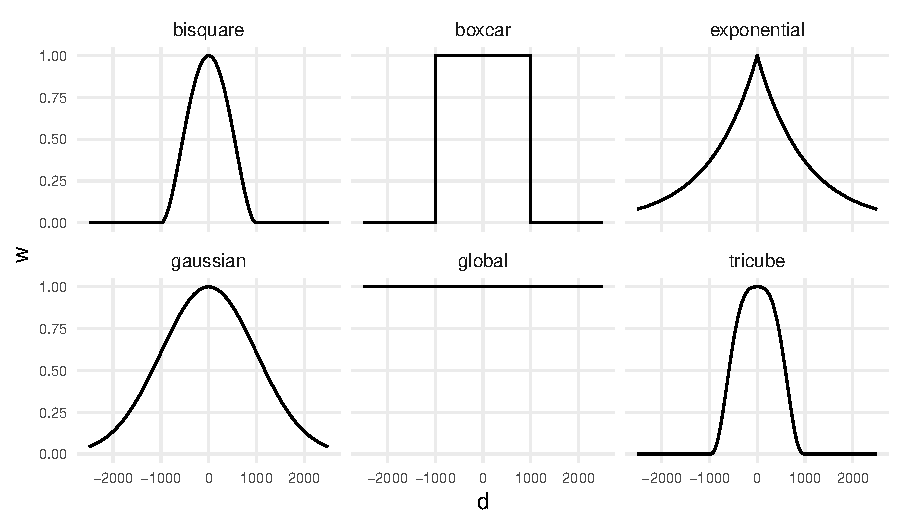
\includegraphics{fig/kernel.pdf}
    \label{fig:kernel}
    \par SOURCE: The Author (2021), based on \textcite{Gollini2013}.
\end{figure}

In addition to the different types of kernel functions, the GWR has multiple configurations based on the type of regression: negative binomial (GWNBR), Poisson (GWPR) and Gaussian, which is the basic form of linear GWR described on  \autoref{eq:gwr}. The GWNBR and GWPR models were used by \textcite{Obelheiro2019}; \textcite{Obelheiro2020} and \textcite{Yu2017} to study the impacts of the built environment on the occurrence of road crashes inside urban areas. % cite Li et al, Xu huang, Gomes as another examples. It wasn't possible to find gwr applications of intermediate outcomes of road safety level, like speeding.

In conclusion, GWR is a method that enables the exploration of findings that might otherwise be missed if only a global regression method is applied. It is always important to really check if the GWR model will describe the data better than a global regression model comparing the results from both. All the process of constructing a GWR model and its parameters for this work is described in section \ref{gwm}.

% ----------------------------------------------------------------------------------

\chapter{METHODS}

\section{NATURALISTIC DATA COLLECTION}

\section{DATA PROCESSING}

\section{GEOGRAPHICALLY WEIGHTED MODEL} \label{gwm}

% ----------------------------------------------------------------------------------

\chapter{ANALYSIS AND RESULTS}

% ----------------------------------------------------------------------------------

\chapter{CONCLUSIONS}
